\section{Dual-Feed Antenna}
\label{sec:tech_sol_ant3}
\begin{figure}[htbp]
    \begin{subfigure}[b]{0.49\linewidth}
        \centering
        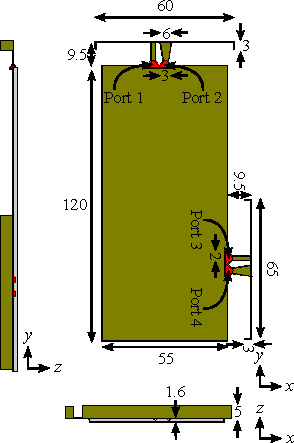
\includegraphics{img/tech_sol/nonresonant/technical}
        \caption{Technical drawing. Unit: mm.}
        \label{fig:ant3technical}
    \end{subfigure}
    \hfill
    \begin{subfigure}[b]{0.49\linewidth}
        \centering
        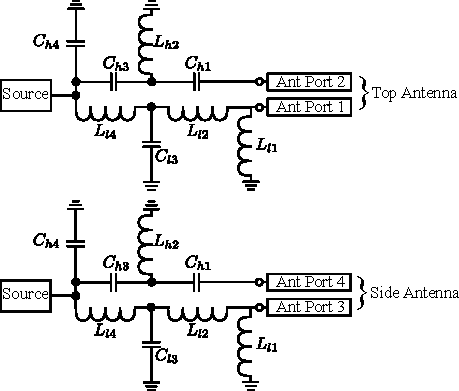
\includegraphics{img/tech_sol/nonresonant/schematic_tuning}\\[0cm]
        \caption{Tuning/matching circuit.}
    \end{subfigure}
    \par\bigskip
        \begin{subfigure}[b]{\linewidth}
        \centering
        \footnotesize
        \begin{tabular}{|l|l|l|l|l|l|l|l|l|}
            \hline
                         & $L_{l1}$       & $L_{l2}$        & $C_{l3}$      & $L_{l4}$       & $C_{h1}$       & $L_{h2}$      & $C_{h3}$      & $C_{h4}$    \\
            \hline
            Top antenna  & \SI{14,34}{nH}  & \SI{25}{nH}  & \SI{2,9}{pF} & \SI{5,51}{nH} & \SI{1,2}{pF} & \SI{7,80}{nH} & \SI{5}{pF} & \SI{2.4}{pF} \\
            Side antenna & \SI{10,49}{nH}  & \SI{15,93}{nH}  & \SI{6.1}{pF} & \SI{4.52}{nH} & \SI{0.68}{pF} & \SI{5.17}{nH} & \SI{3.47}{pF} & \SI{2.69}{pF} \\
            \hline
        \end{tabular}
        \caption{Component values}
    \end{subfigure}
    \caption{Technical drawing and tuning circuit for the antenna.  The antennas are built on FR-4 board using \SI{35}{\micro\meter} copper. There is a matching circuit as shown for each of the two feeds.}
    \label{fig:ant3techschem}
\end{figure}


%Intro to design + references. 
This design is an inherently non-resonant capacitive coupling element antenna based on the one shown in \cite{valkonen2013inherently}. The antenna presented in \cite{valkonen2013inherently} does not have any tuning capabilities, nor is it designed for MIMO operation. The antenna is shown in Figure~\ref{fig:ant3techschem}, as seen the antenna is , which enhances the bandwidth and efficiency. The antenna has two feeds, but only a single signal port is used. The signal is split into two branches at the matching network, one for the low band and one for the high band. The novel matching network is also based on \cite{valkonen2013inherently}.

As seen on Figure~\ref{fig:ant3techschem} the matching network is quite complex, this is usually the case for non-resonant CCE antennas, since the antenna structure is simplified greatly compared to other multi-resonant antennas, e.g.\ \cite{Tatomirescu2014AT}, \cite{Zhekov2015} and \cite{Zhang2013Diag}.

% What makes it radiate at 900, 1800, and 2400?
The low band element consists of a non-resonant CCE, where the resonance is dependent on the matching circuit. For this design, the matching is \emph{mostly} performed by $L_{l1}$, $L_{l2}$, $L_{l3}$, $L_{l4}$ and $C_{l4}$. The higher-band is matched by $C_{h1}$, $L_{h2}$, $C_{h3}$ and $C_{h4}$, furthermore there is a natural resonance at \SI{2700}{MHz}, at the trapezoidal feed (Port 2), which extends the frequency of operation. It should also be noted that the low and high band are dependent on every part of the matching network, even though the components a denoted high (h) and low (l). 
 
The surface currents, illustrating how the structure resonates after matching, is shown in Figure~\ref{fig:ant3_sc}.


\begin{figure}[htbp]
   \begin{subfigure}[b]{0.32\linewidth}
        \centering
        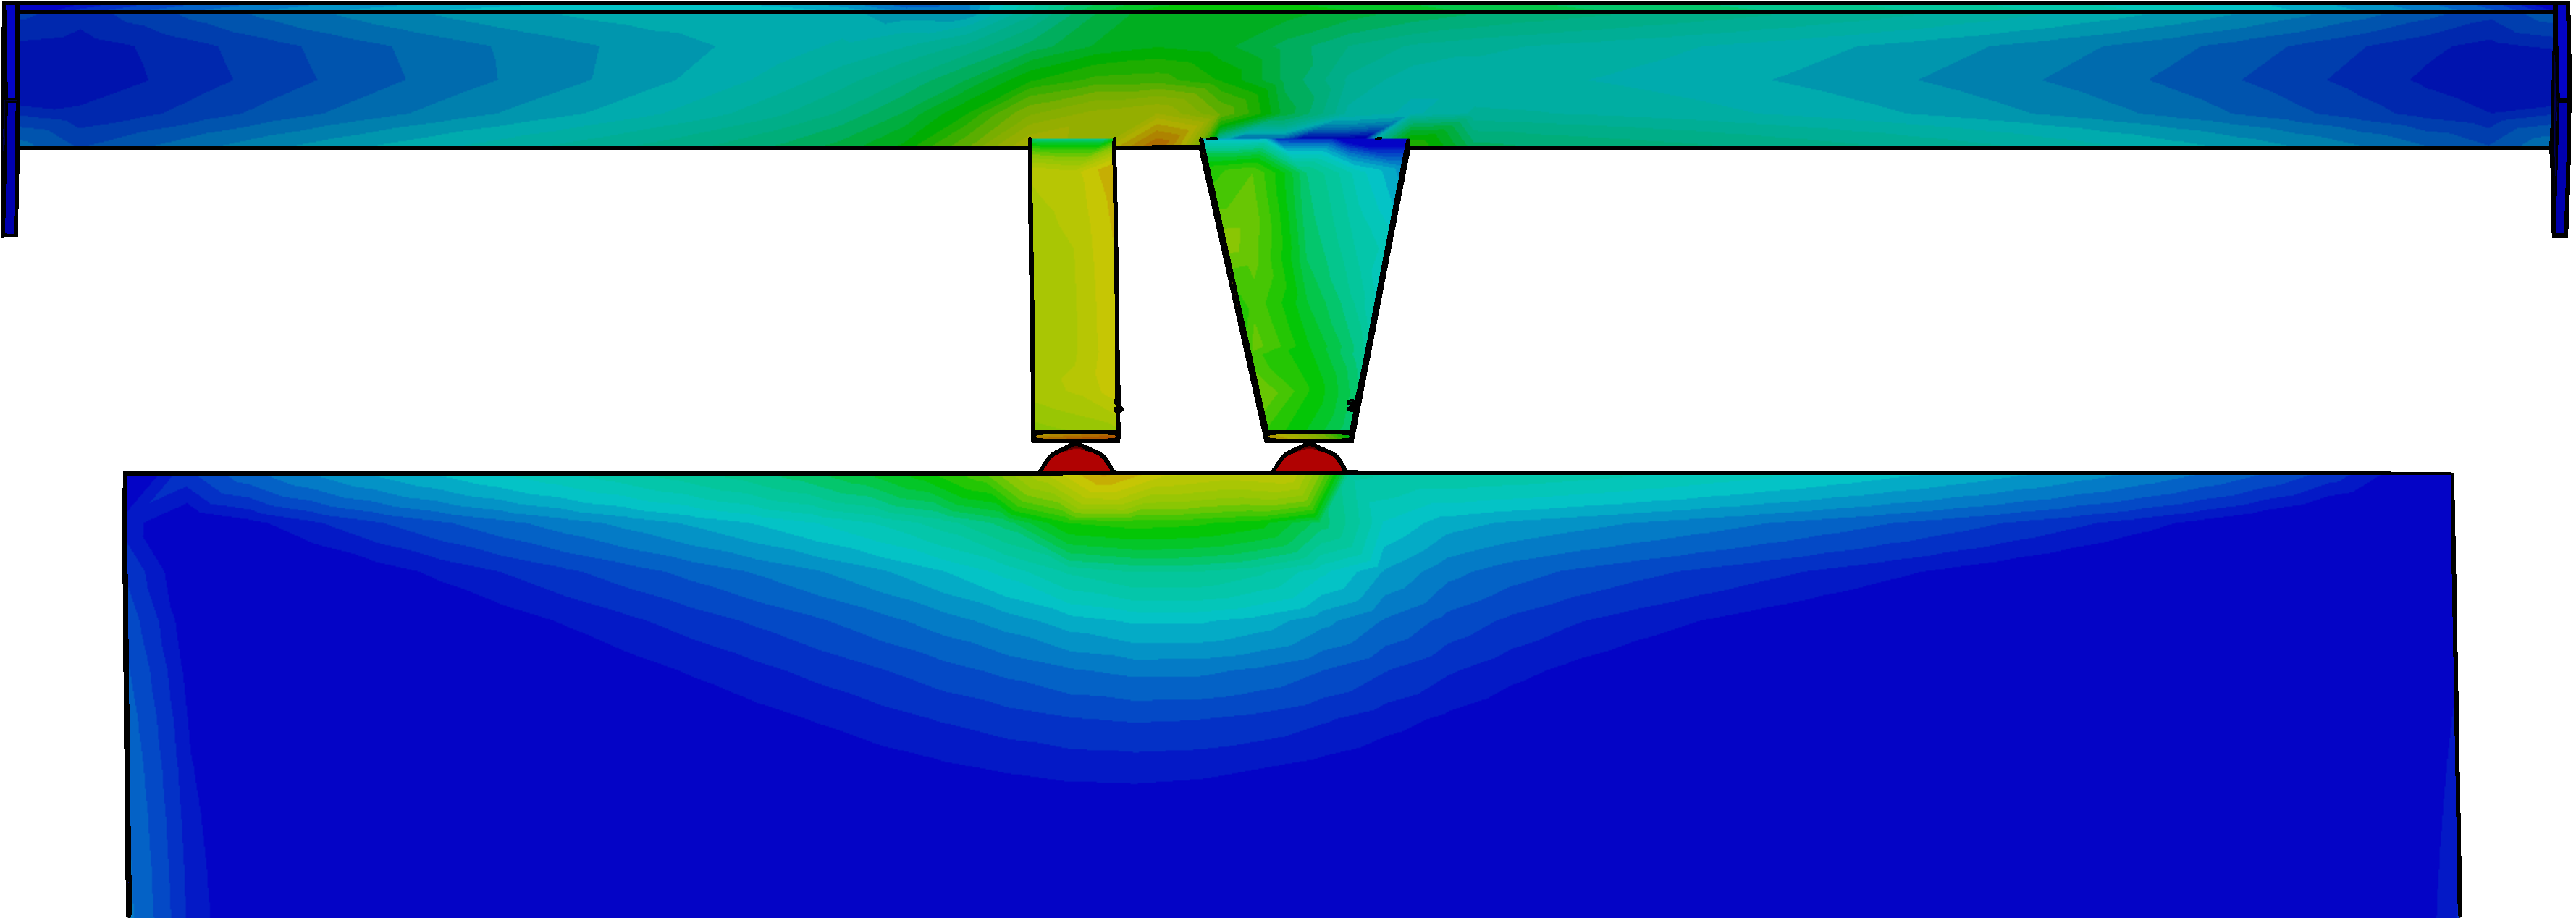
\includegraphics[width=\linewidth]{img/tech_sol/nonresonant/finka-surface-800}
        \caption{Surface current for \SI{800}{MHz}}
        \label{fig:ant3_sc800}
    \end{subfigure}
    \hfill
    \begin{subfigure}[b]{0.32\linewidth}
        \centering
        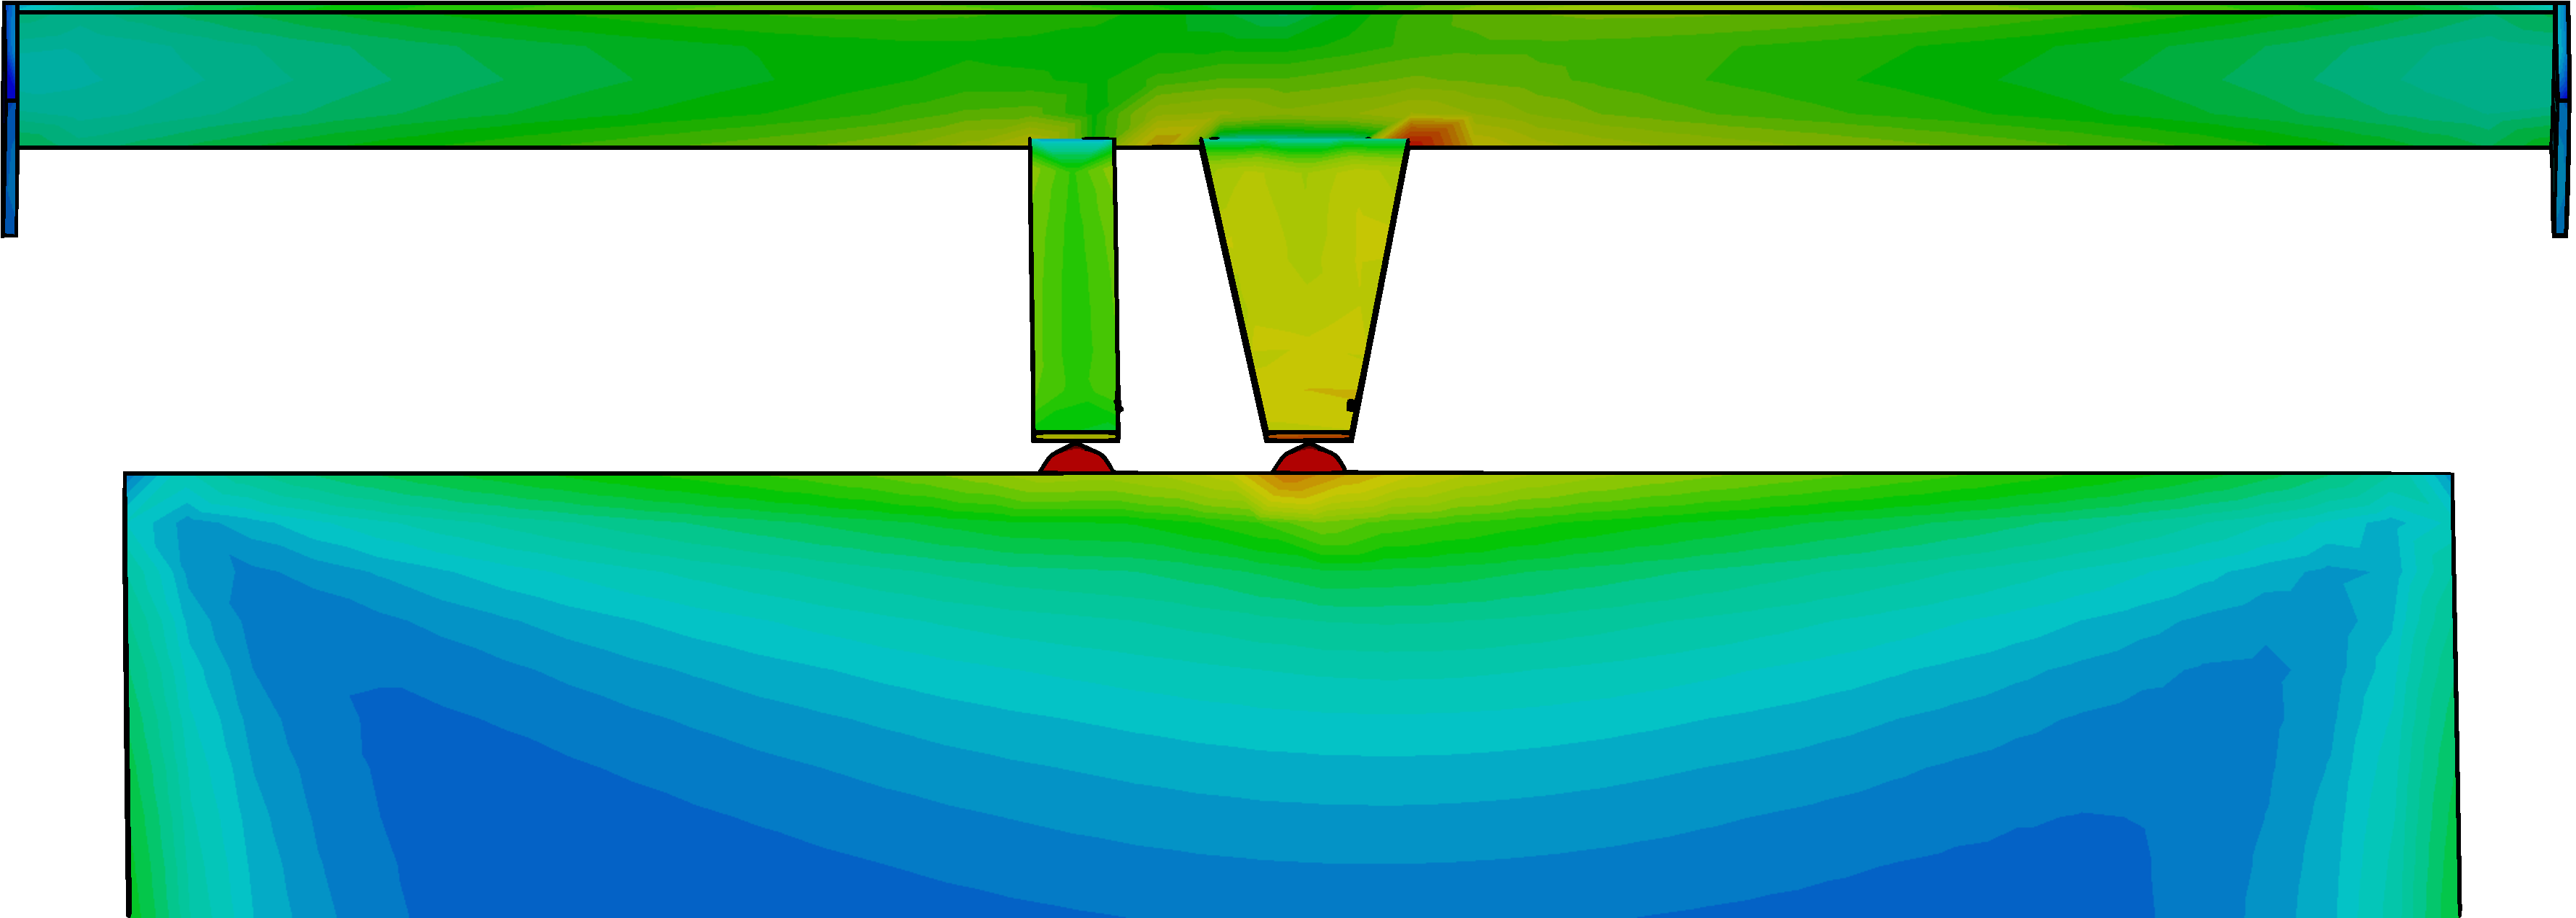
\includegraphics[width=\linewidth]{img/tech_sol/nonresonant/finka-surface-1800}
        \caption{Surface current for \SI{1800}{MHz}}
        \label{fig:ant3_sc1800}
    \end{subfigure}
    \hfill
    \begin{subfigure}[b]{0.32\linewidth}
        \centering
        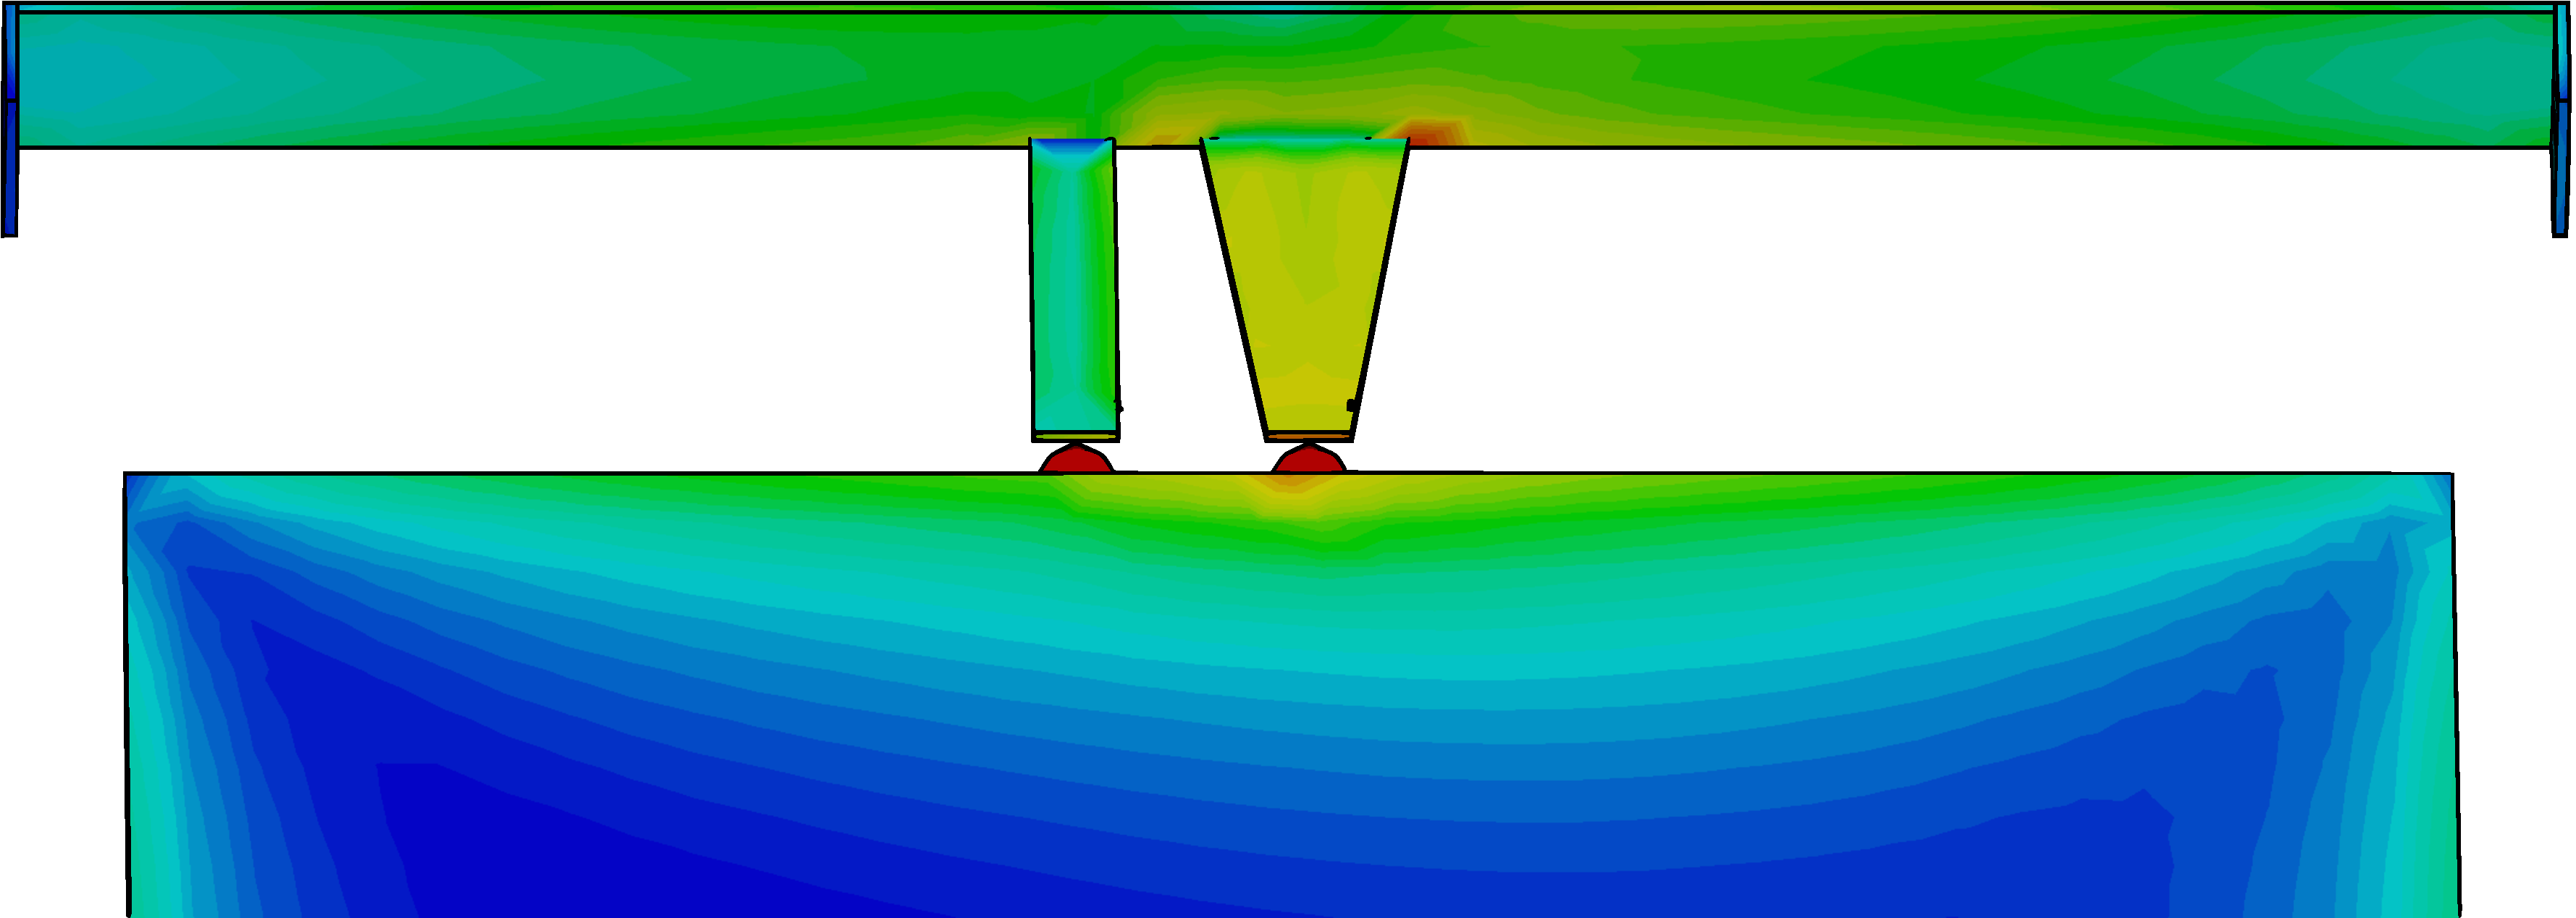
\includegraphics[width=\linewidth]{img/tech_sol/nonresonant/finka-surface-2400}
        \caption{Surface current for \SI{2400}{MHz}}
        \label{fig:ant3_sc2400}
    \end{subfigure}
    \caption{Surface currents}
    \label{fig:ant3_sc}
\end{figure}

%%%Her fra%%%%%%

\begin{figure}[htbp]
    \centering
    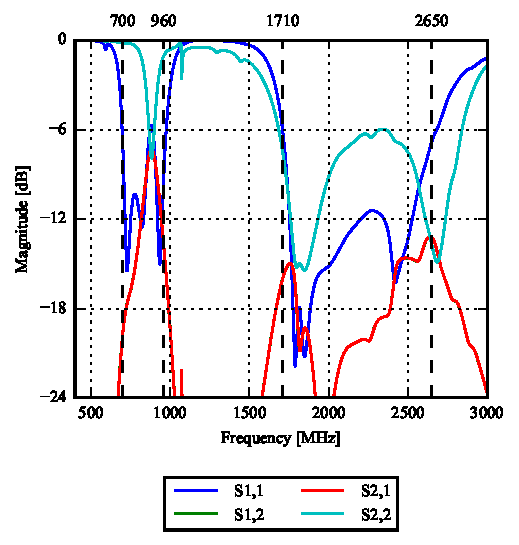
\includegraphics{img/tech_sol/nonresonant/simulation/freespace/Spara-static}
    \caption{$S$-parameters with $C_{l3} = \SI{2.9}{pF}$ and $s\_C_{h1} = \SI{0.68}{pF}$}
    \label{fig:ant3sparams}
\end{figure}

The $S$-parameters for both the top and the side antenna are shown in Figure~\ref{fig:ant3sparams}. The tuning capacitors are chosen, for a maximum bandwidth with values: $C_{l3} = \SI{2.9}{pF}$ and $s\_C_{h1} = \SI{0.68}{pF}$. At this position the top antenna (port 1) covers the entire low and high band. The side antenna covers much less and must be tuned to cover the whole low band. However, the high band is covered. 

% Sweep description %%
It is seen that the isolation at low frequencies is only around \SI{8}{dB}. This may cause problems when using the antennas for MIMO operation. The low isolation is most likely due to the way the CCE antenna resonates, since it uses the chassis as the resonator \cite{ilvonen2014design}.

This design provides high bandwidth, covering most desired bands for both antennas. In this design, the top antenna would be used as the main antenna and the side antenna would be used for diversity, carrier aggregation, and MIMO operation. 

\begin{table}[htbp]
    \centering
    \begin{tabular}{|l|l|r|r|r|}
        \hline
        Antenna & Band & Start [MHz] & Stop [MHz] & Bandwidth [MHz] \\
        \hline
        Top     & Low  & 689         & 1087       & 398 \\
        Side    & Low  & 670         & 911        & 241 \\
        \hline
        Top     & High & 1714        & 2704       & 990 \\
        Side    & High & 1410        & 2845       & 1435 \\
        \hline
    \end{tabular}
    \caption{Maximum bandwidth obtained in the low and high band for the top and the side antenna, respectively.}
    \label{tab:bw_sol3}
\end{table}

% Bandwidth
The bandwidth of each antenna is shown in Table~\ref{tab:bw_sol3}. It is clear that both antennas fulfill the requirements of tunable impedance bandwidth seen in the requirement specification, Section~\ref{cha:reqspec}. Below are the tuned $S$-parameters shown. The fixed antenna will be set to the maximum capacitor value, since this yields the best match.  

\begin{figure}[htbp]
    \begin{subfigure}{0.49\linewidth}
        \centering
        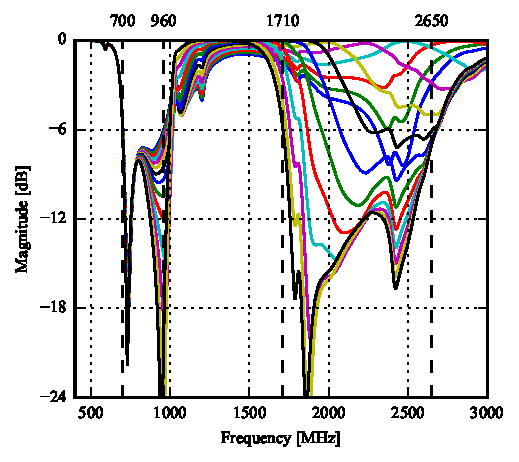
\includegraphics{img/tech_sol/nonresonant/simulation/freespace/s11_top_sweep.pdf}
        \caption{$S_{11}$, sweeping $C_{l3}$ and fixing $s\_C_{h1}$.}
    \end{subfigure}
    \hfill 
    \begin{subfigure}{0.49\linewidth}
        \centering
        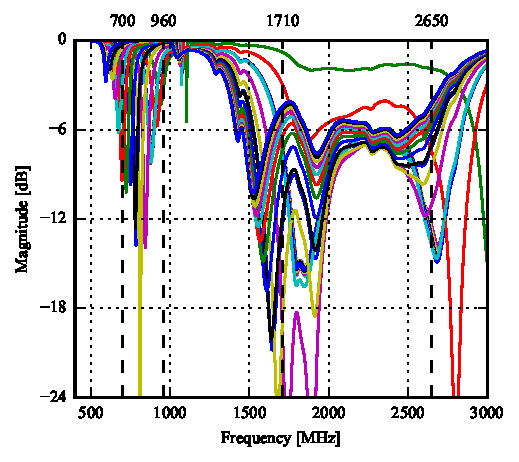
\includegraphics{img/tech_sol/nonresonant/simulation/freespace/s22_side_sweep.pdf}
        \caption{$S_{22}$, sweeping $s\_C_{h1}$ and fixing $C_{l3}$.}
    \end{subfigure}
    \\
    \begin{subfigure}{0.49\linewidth}
        \centering
        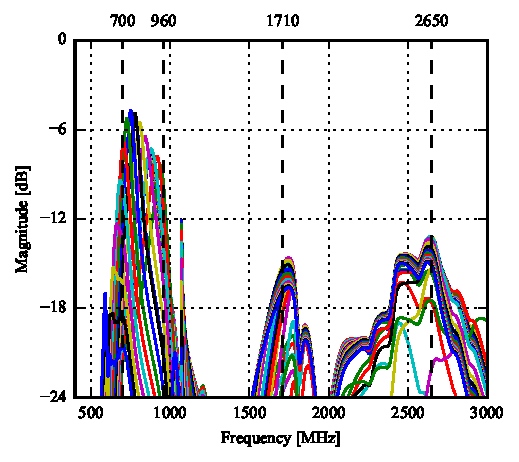
\includegraphics{img/tech_sol/nonresonant/simulation/freespace/s12_top_sweep.pdf}
        \caption{$S_{21}$, sweeping $C_{l3}$ and fixing $s\_C_{h1}$.}
    \end{subfigure}
    \hfill
    \begin{subfigure}{0.49\linewidth}
        \centering
        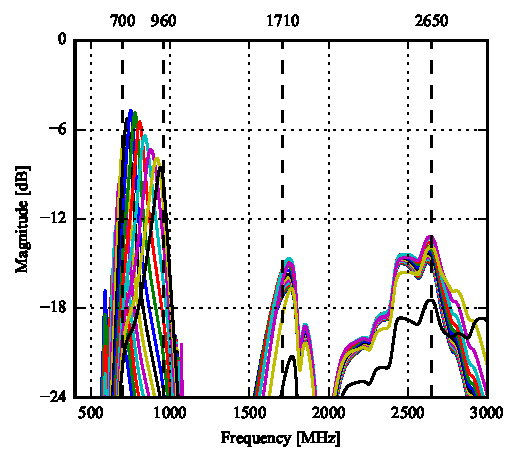
\includegraphics{img/tech_sol/nonresonant/simulation/freespace/s21_side_sweep.pdf}
        \caption{$S_{21}$, sweeping $s\_C_{h1}$ and fixing $C_{l3}$.}
    \end{subfigure}
    \caption{Parameter sweeps when tuning the shunt capacitor of each antenna, $C_{l3}$ and $s\_C_{h1}$ for port 1 and 2, respectively. Port 1 is the top antenna and port 2 is the side antenna.}
    \label{fig:ant3sweeps}
\end{figure}

% Correlation
\begin{figure}[htbp]
    \centering
    \begin{subfigure}{0.49\linewidth}
        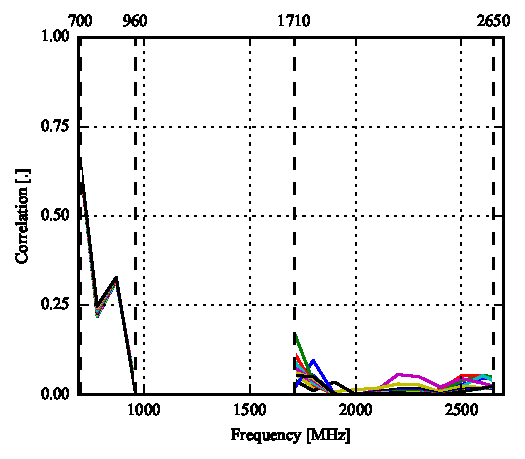
\includegraphics{img/tech_sol/nonresonant/simulation/freespace/sweep_top_corr}
        \caption{Sweeping $C_{l3}$ and fixing $s\_C_{h1}$.}
    \end{subfigure}
    \hfill
    \begin{subfigure}{0.49\linewidth}
        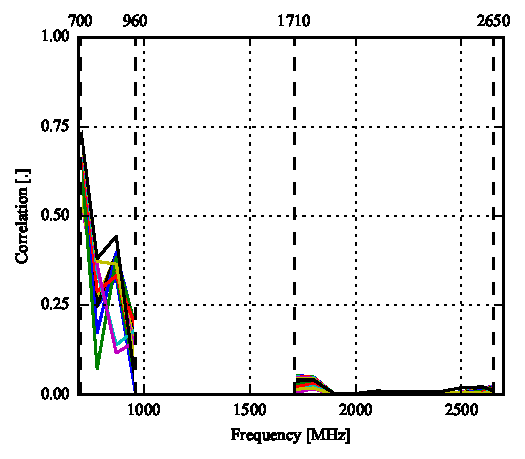
\includegraphics{img/tech_sol/nonresonant/simulation/freespace/sweep_side_corr}
        \caption{Sweeping $s\_C_{h1}$ and fixing $C_{l3}$.}
    \end{subfigure}
    \caption{Correlation between antennas then sweeping tuning capacitors. Here, $C_{l3}$ and $s\_C_{h1}$ are the tuning capacitor for the top and side antenna, respectively.}
    \label{fig:corr_sol3}
\end{figure}

%%
The correlation between the top an side antennas are shown in Figure~\ref{fig:corr_sol3} when sweeping the tuning capacitors. Here it is seen that the correlation is low for the high band, while being quite high in the lowest part of the low band.  

% Efficiency
\begin{figure}[htbp]
    \centering
    \begin{subfigure}{0.49\linewidth}
        \centering
        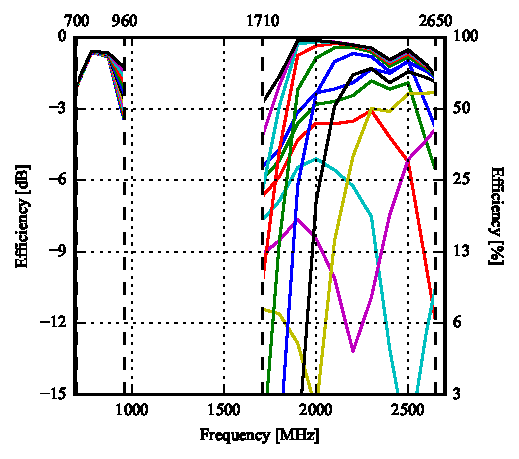
\includegraphics{img/tech_sol/nonresonant/simulation/freespace/Efficiency_AC2/efficiency-ac2-top.pdf}
        \caption{Top antenna. Sweeping $C_{l3}$, fixing $s\_C_{h1}$.}
    \end{subfigure}
    \hfill
    \begin{subfigure}{0.49\linewidth}
        \centering
        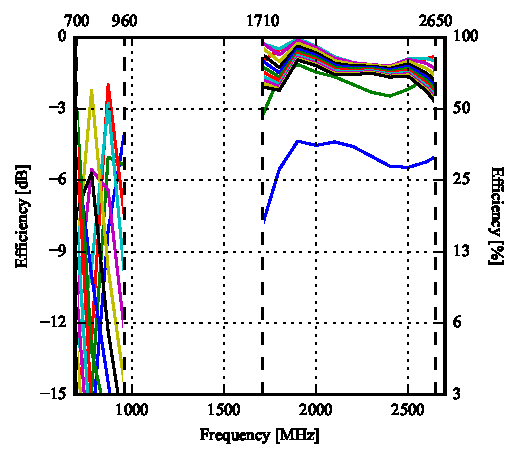
\includegraphics{img/tech_sol/nonresonant/simulation/freespace/Efficiency_AC3/efficiency-ac3-side.pdf}
        \caption{Side antenna. Sweeping $s\_C_{h1}$, fixing $C_{l3}$.}
    \end{subfigure}
    \caption{Efficiency for each antenna when sweeping the tuning capacitors. Here, $C_{l3}$ and $s\_C_{h1}$ are the tuning capacitor for the top and side antenna, respectively.}
    \label{fig:eff_sol3}
\end{figure}

%%
The total system efficiency sweep, is shown in Figure~\ref{fig:eff_sol3}. It is seen that the top antenna is very efficient, where the lowest efficiency is around \SI{-3}{dB} for the low band and much higher for the high band. The side antenna has a total efficiency greater than \SI{-6}{dB} for the low band and higher than \SI{-3}{dB} for the high band, except for a single capacitor value.


